% !TeX spellcheck = hu_HU
\documentclass[12pt,a4paper]{article}
\usepackage[utf8]{inputenc}
\usepackage{cmap}
\usepackage[T1]{fontenc}
\usepackage[magyar]{babel}
\usepackage{amsmath}
\usepackage{amsfonts}
\usepackage{amssymb}
\usepackage{graphicx}

\usepackage{outlines}
\usepackage{hyperref}

\hyphenpenalty=10000

\begin{document}

\begin{center}
	\huge
	Numerikus módszerek I\\
	\vspace{1mm}
	\LARGE
	Gyakorlat jegyzet\\
	\vspace{5mm}
	\large
	Készült Bozsik József előadásai és gyakorlatai alapján\\
	\vspace{5mm}
	Sárközi Gergő, 2021-22-2. félév\\
	Nincsen lektorálva!
\end{center}

\tableofcontents

\pagebreak

\section{Gépi számábrázolás, hibaszámítás}

\subsection{Gépi számok, lebegőpontos számábrázolás egy modellje}

\begin{outline}
	\1 Normalizált lebegőpontos szám: $a = \pm m * 2^k = \pm [m_1 ... m_t | k]$
		\2 $m$: mantissza, hossza $t$, $m=\sum_{i=1}^{t} m_i*2^{-i}$ \; ($m_1=1$; $m_i \in \{0,1\}$)
		\2 $k$: karakterisztika, $k^- \le k \le k^+$
	\1 Gép számok halmaza: $M=M(t,k^-,k^+)$ \; ($k^-,k^+ \in \mathbb{Z}$ és $t \in \mathbb{N}$)
		\2 $M(t,k^-,k^+) = \{\pm 2^k * \sum_{i=1}^{t} m_i * 2^{-i} \} \cup \{0\}$
		\2 Gyakran hozzávesszük: $+\infty, -\infty, NaN$
	\1 Gép számok halmazának tulajdonságai:
		\2 $\frac{1}{2} \le m < 1$ \; és \; $M$ szimmetrikus 0-ra
		\2 $\epsilon_0$: legkisebb pozitív elem: $\epsilon_0 = [100...0|k^-] = \frac{1}{2} * 2^{k^-} = 2^{k^- - 1}$
		\2 $M_\infty$: legnagyobb elem: $M_\infty = [111...1|k^+] = (1-2^{-t}) * 2^{k^+}$
		\2 $M$-ben az $1$ után következő gépi szám és az $1$ különbsége:\\
		$\epsilon_1 = [100...01|1] - [100....00|1] = 2^{-t} * 2^1 = 2^{1-t}$
		\2 $|M|$: $M$ számossága: $|M|=2*2^{t-1}*(k^+ - k^- + 1) + 1$
\end{outline}

\subsection{Valós számok ábrázolása gépi számmal}

\begin{outline}
	\1 Ábrázolható számok tartománya: $\mathbb{R}_M = \{x \in \mathbb{R}: |x| \le M_\infty\}$
	\1 Input függvény, $fl : \mathbb{R}_M \to M$: $x$-hez $\widetilde{x}$-et rendel
		\2 $\widetilde{x}$ az $x$-hez legközelebbi gépi szám, kerekítés szabályai szerint
		\2 $fl(x) = \begin{cases}
		0 &\text{ ha } |x| < \epsilon_0\\
		\widetilde{x} &\text{ ha } \epsilon_0 \le |x| \le M_\infty\\
		+\infty &\text{ ha } |x| > M_\infty
		\end{cases}$
\end{outline}

\subsubsection{Hibakorlátok}

\begin{outline}
	\1 Input hiba: $\forall x \in \mathbb{R}_M: |x-fl(x)| \le \begin{cases}
		\epsilon_0 \;\;\;\;\;\;\;\;\;\;\;\;\;\;\;\;\; \text{ha} \;\; |x| < \epsilon_0 \\
		0.5*|x|*\epsilon_1 \;\; \text{ha} \;\; \epsilon \le |x| \le M_\infty
	\end{cases}$
	\1 Abszolút hibakorlát: $\Delta_x = 0.5 * 2^k * 2^{-t}$
	\1 Relatív hibakorlát: $\delta_x = 2^{-t}$
\end{outline}

\pagebreak

\subsubsection{Input függvény a gyakorlatban}

\begin{outline}
	\1 Feladat: $M(5,-4,4)$-ben $fl(10,85) = \; ?$
	\1 Első lépés: szám átalakítása 2-es számrendszerbe
		\2 Táblázatban lehet egyből törtet is átalakítani, pl. $1/6$
		\2 Kezdő nullákat elhagyjuk, a karakterisztikát annyival eltoljuk

\begin{table}[h]
	\centering
	\begin{tabular}{|c|c|c|c|c|}
		\hline
		10 & 5 & 2 & 1 & 0 \\
		\hline
		$(:2)$ & 0 & 1 & 0 & 1 \\
		\hline
		$1010_{(2)}$ & $\leftarrow$ & $\leftarrow$ & $\leftarrow$ & $\leftarrow$ \\
		\hline
	\end{tabular}
	\caption{Egészrész binárisba alakítása}
\end{table}

\begin{table}[h]
	\centering
	\begin{tabular}{|c|c|c|c|c|c|c|c|}
		\hline
		85 & 70 & 40 & 80 & 60 & 20 & 40 & 80 \\
		\hline
		$(*2)$ & 1 & 1 & 0 & 1 & 1 & 0 & 0 \\
		\hline
		$\approx 0.11011_{(2)}$ & $\rightarrow$ & $\rightarrow$ & $\rightarrow$ & $\rightarrow$ & $\rightarrow$ & $\rightarrow$ & $\rightarrow$ \\
		\hline
	\end{tabular}
		\caption{Törtrész binárisba alakítása}
\end{table}

		\2 Eredmény: $10,85 \approx 1010.11011_{(2)} = 1010.1|1011_{(2)}$
	\1 Második lépés: kerekítés
		\2 Eredmény: $fl(10,85) = [10110|4] = \frac{22}{32} * 2^4 = 11$
	\1 Harmadik lépés: hibaszámolás: $|10,85 - fl(10,85)| = 0,15$
\end{outline}

\subsection{Gépi számok összeadása}

\begin{outline}
	\1 Azonos karakterisztikájú számok összeadása:
	mantisszák összeadása, szükség esetén normalizálás (kerekítéssel)
	\1 Eltérő karakterisztikájú számok összeadása:
	kisebbik karakterisztikát a nagyobbikhoz igazítjuk (kerekítünk, ha kell), majd normál összeadás
	\1 Van rá példa: $b \ne 0 \wedge a \oplus b = a$
		\2 pl. $b$ karakterisztikája $\le$ $a$ karakterisztikája + mantissza + 1\\
		$[10011|4] \oplus [10010|-2] \implies 0.10010_{(2)}*2^{-2} = 0.00000010010_{(2)}*2^4$
	\1 Van rá példa: asszociativitás nem teljesül
		\2 pl. (nagy+kicsi)+kicsi \; vs \; nagy+(kicsi+kicsi)
	\1 ZH-ban részletesen le kell vezetni pl. a karakterisztika váltást
\end{outline}

\pagebreak

\subsection{Hibaszámítás elemei}

\subsubsection{Hibák jellemzése}

\begin{outline}
	\1 Legyen $A$ egy pontos érték, $a$ pedig egy közelítő érték
	\1 $\Delta a = A - a$: közelítő érték pontos hibája
	\1 $|\Delta a| = |A - a|$: közelítő érték abszolút hibája
	\1 $\Delta_a \ge |\Delta a|$: közelítő érték abszolút hibakorlátja
	\1 $\delta a = \frac{\Delta a}{A} \approx \frac{\Delta a}{a}$: közelítő érték relatív hibája
	\1 $\delta_a \ge |\delta a|$: közelítő érték relatív hibakorlátja
	\1 Kerekítés abszolút hibakorlát: 2 tizedesjegyes kerekítés esetén $0.005$
\end{outline}

\subsubsection{Alapműveletek hibakorlátai}

\begin{outline}
	\1 Tétel: alapműveletek hibakorlátai
		\2 $\Delta_{a \pm b} = \Delta_a + \Delta_b$ \;\;\;\;\;\;\;\;\;\;\;\;\;\;\;\;\;\;\;\;
		$\delta_{a \pm b} = (|a|\delta_a+|b|\delta_b) \;/\; |a \pm b|$
		\2 $\Delta_{a * b} = |b|\Delta_a + |a|\Delta_b$ \;\;\;\;\;\;\;\;\;\;\;\;\;\;
		$\delta_{a * b} = \delta_a + \delta_b$
		\2 $\Delta_{a / b} = (|b|\Delta_a + |a|\Delta_b) \;/\; b^2$ \;\;\;\;\;
		$\delta_{a / b} = \delta_a + \delta_b$
	\1 Két esetben van nagyságrendileg nagyobb hiba, ezeket érdemes elkerülni:
		\2 $\delta_{a \pm b}$: közeli számok kivonása egymásból
		\2 $\Delta_{a/b}$: kicsi számmal osztás
\end{outline}

\subsubsection{Függvényérték hibája, kondíciószáma}

\begin{outline}
	\1 Függvényérték relatív hibája: Ha $\Delta_a$ kicsi, akkor $\delta_{f(a)} = \frac{|a||f'(a)|}{|f(a)|}*\delta_a$
	\1 $f$ függvény $a$-beli kondíciószáma: $c(f,a)=\frac{|a||f'(a)|}{|f(a)|}$
\end{outline}

\pagebreak

\section{Mátrixokról általánosságban}

\begin{outline}
	\1 $a_{ij}$ jelentése: i. sor, j. oszlop az $A$ mátrixban
	\1 $\mathcal{U}$: felső háromszögmátrixok
	\1 $\mathcal{L}_1$: alsó háromszögmátrixok; főátlójukban csupa $1$-es van
	\1 $A^T$ jelentése: főátlóra tükrözés
	\1 Szimmetrikus mátrix: $A = A^T$
	\1 Sorokra/oszlopokra szigorúan diagonálisan domináns mátrix: főátlóban lévő elemek abszolútértéke szigorúan nagyobb, mint az adott sorban/oszlopban lévő elemek abszolútértékének összege (átlót nem beleszámítva)
\end{outline}

\subsection{Pozitív definit mátrix definíció}

\begin{outline}
	\1 Legyen szimmetrikus (TODO ebben a tárgyban ez feltétel vagy sem?)
	\1 Ezek közül legyen egy igaz (ha egy igaz, az akkor az összes is):
		\2 $<Ax,x> = x^TAx>0$ bármely $0 \ne x \in \mathbb{R}^n$ esetén
		\2 minden főminorjának determinánsa pozitív
		\2 minden sajátértéke pozitív
	\1 Példa pozitív definit mátrixra: diagonális és minden eleme pozitív
\end{outline}

\subsection{Ortogonális mátrix, ortonormált rendszer}

\begin{outline}
	\1 Ortogonális mátrix: $Q^T = Q^{-1}$
		\2 Oszlopaik, mint vektorok, ortonormált rendszert alkotnak
		\2 Ortogonális mátrixok szorzata is ortogonális
	\1 Ortonormált rendszer: $<q_i,q_j> = \begin{cases}
	0 & $\text{ ha }$ i \ne j\\
	1 & $\text{ ha }$ i = j
	\end{cases}$
		\2 Ortogonális rendszer: $i=j$ esetében lehet bármi, nem csak $1$
\end{outline}

\subsection{Sajátérték számolás}

\begin{outline}
	\1 $|A - \lambda I| = 0$, azaz főátlón mindenhol kivonunk $\lambda$-t, kiszámoljuk a paraméteres determinánst és megoldunk egy egyenlőséget ($det = 0$)
\end{outline}

\pagebreak

\subsection{Determináns számolás}

\begin{outline}
	\1 $1 \times 1$ mátrix: a szám maga
	\1 $\begin{bmatrix} a & b \\ c & d \end{bmatrix}$ mátrix: $ad - bc$
	\1 $\begin{bmatrix} a & b & c \\ d & e & f \\ g & h & i \end{bmatrix}$ mátrix:
	$a * \begin{vmatrix} e & f \\ h & i \end{vmatrix}
	- b * \begin{vmatrix} d & f \\ g & i \end{vmatrix}
	+ c * \begin{vmatrix} d & e \\ g & h \end{vmatrix}$
		\2 Lehet sor helyett oszlop szerint is kibontani
	\1 Determináns tartó műveletek:
		\2 egy sorhoz hozzáadni egy másik sor konstans-szorosát
	\1 Determináns meg kell szorozni $(-1)^n$-szer: oszlop, sorcserék száma
	\1 Kapcsolat önmagával:
		\2 $\det(A^T) = \det(A)$
		\2 $\det(AB) = \det(A) \det(B)$
		\2 $\det(A^{-1}) = 1 / \det(A)$
		\2 $n \times n$-es mátrix: $\det(cA) = c^n * \det(A)$
	\1 Háromszög mátrix: determináns a főátlón lévő elemek szorzata
	\1 Főminorok: egy mátrix bal felső almátrixjainak a determinánsai
		\2 $D_k$ a $k \times k$ bal felső részmátrix determinánsa
\end{outline}

\subsection{Invertálás}

\begin{outline}
	\1 Diagonális mátrix: (főátló) elemeinek reciproka
	\1 $A^{-1} = \begin{bmatrix} a & b \\ c & d \end{bmatrix}^{-1} =
	\frac{1}{det(A)} \begin{bmatrix} d & -b \\ -c & a \end{bmatrix}$
	\1 $\begin{bmatrix} a & b & c \\ 0 & d & e \\ 0 & 0 & f \end{bmatrix}^{-1}
	= \begin{bmatrix} 1/a & -b/(ad) & (be-cd)/(afd) \\ 0 & 1/d & -e/(fd) \\ 0 & 0 & 1/f \end{bmatrix}$
		\2 Alsó háromszögmátrix: ugyan így
\end{outline}

\pagebreak

\section{Gauss-elimináció (GE)}

\begin{outline}
	\1 Alak: [A|b]
	\1 Első rész: főátló alatt nullázás, balról jobbra
		\2 Ezután már egyből lehet determinánst számolni
	\1 Második rész: főátló fölött nullázás, jobbról balra, sor osztása magával
		\2 Kihagyható: egyenletrendszerrel enélkül is megoldható az $Ax=b$
	\1 Nullázás: a pillanatnyi sor konstans-szorosát hozzáadjuk egy másikhoz
	\1 Inverz számolás: $b$ helyett az identitásmátrix legyen a jobb oldalon.\\
	Ekkor amikor bal oldalon identitásmátrix van: jobb oldalon az inverz.
	\1 Sorcsere: nem változik a megoldás
	\1 Oszlopcsere: a megoldás komponensei cserének megfelelően változnak
	\1 Főátlón 0 van, alatta/felette nem: oszlop/sorcsere kell
	\1 Nincs megoldás: ha bal oldalon 0-k vannak a sorban, jobb oldalon nem
	\1 Függő paraméter: ha egy sorban csak 0-k vannak mindkét oldalt
\end{outline}

\begin{figure}[h!]
	\centering
	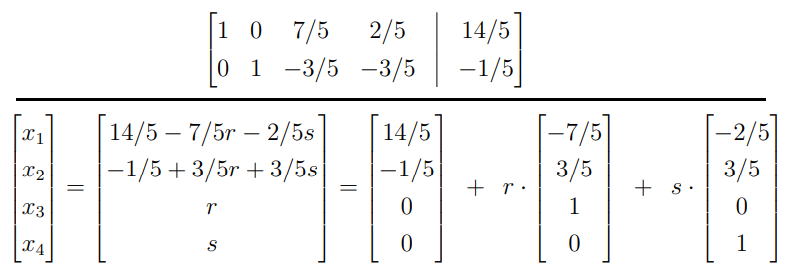
\includegraphics[width=0.7\linewidth]{ge-sor-nulla}
\end{figure}

\subsection{Főelemkiválasztás}

\begin{outline}
	\1 Részleges főelemkiválasztás: adott oszlopban maximális abszolút értékű elem (sor) kiválasztása (ami a főátlón vagy az alatt van), áthelyezése a főátlóra, és a többi sor azzal való eliminálása
	\1 Teljes főelemkiválasztás: részleges főelemkiválasztás, csak bármelyik oszlopból választunk (de mindig csak a jobb alsó részmátrixból)	
\end{outline}

\pagebreak

\section{$LU$ felbontás ($A = LU$, ahol $L \in \mathcal{L}_1$ és $U \in \mathcal{U}$)}

\begin{outline}
	\1 Felhasználás: $Ax=b$ helyett $Ly=b$ (alsó $\Delta$) és $Ux=y$ (felső $\Delta$)
\end{outline}

\subsection{Gauss-eliminációval (GE-vel)}

\begin{outline}
	\1 $L_{n-1} * ... * L_2 * L_1 * A = U \implies
	A = L_1^{-1} * L_2^{-1} * ... * L_{n-1}^{-1} * U = LU$
	\1 Minden GE lépés egy $L_i \in \mathcal{L}_1$, elemei: hányszorost adtunk a sorhoz
	\1 $L_i$ invertálásakor az elemek előjelet cserélnek, ekkor elemek: $\frac{\text{adott sorbeli érték}}{\text{elemináló sor értéke}}$
	\1 Tömör írásmód: nem hozunk létre $L_i$ mátrixokat, hanem a GE-ben használt mátrix alsó részét vastag vonallal leválasztjuk és oda írjuk be a végső $L$ értékeit, folyamatosan, ahogy kiszámoljuk őket
\end{outline}

\subsection{Létezés (ami $\ne$ LER megoldhatóság)}

\begin{outline}
	\1 GE végrehajtható sor- és oszlopcsere nélkül $\implies$ létezik $LU$ felbontás
	\1 $D_k$ főminorok $\ne 0 \implies$ létezik $LU$ felbontás (és $u_{kk} \ne 0$)
	\1 $\det(A) \ne 0 \implies$ az $LU$ felbontás egyértelmű
\end{outline}

\subsection{$LU$ mátrixok közvetlen kiszámolása (GE nélkül)}

\begin{outline}
	\1 Írjuk fel az $L,U$ mátrixokat változókkal (minden elem $0$ vagy egy változó)
		\2 Segítség: $U$ és $A$ első sora megegyezik
		\2 Segítség: $A$ első oszlopa leosztva $a_{11}$-gyel egyezik $L$ első oszlopával
	\1 Egy jó sorrendben (lásd kép) számoljuk ki a változókat: mátrixszorzás eredményét tudjuk, vissza kell fejtenünk a változókat
		\2 Ellentmondás $\implies$ az $LU$ felbontás nem létezik
\end{outline}

\begin{figure}[h!]
	\centering
	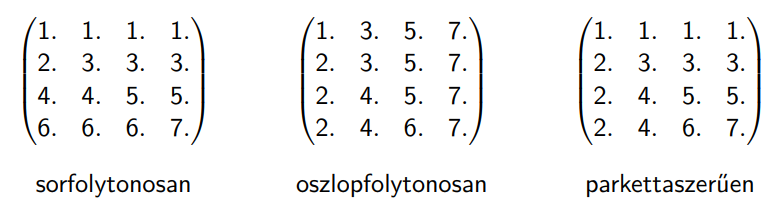
\includegraphics[width=0.8\linewidth]{lu-sorrend}
\end{figure}

\pagebreak

\section{$LDU$ felbontás ($L \in \mathcal{L}_1$, $U \in \mathcal{U}_1$, $D$ diagonális)}

\begin{outline}
	\1 Előállítás $LU$ felbontásból: $A = L \widetilde{U} = LD * (D^{-1} \widetilde{U}) = LDU$
		\2 $\widetilde{U}$ főátlóját átmásoljuk $D$-be, helyére $1$-esek kerülnek
		\2 $\widetilde{U}$ minden többi elemét leosztjuk $\widetilde{U}$ azonos sorának főátlóbeli elemével
		\2 Így megkaptuk az $U$ mátrixot, $L$ mátrixot pedig békén hagyjuk
\end{outline}

\subsection{Szimmetrikus $A$ mátrix, $LDL^T$ felbontás}

\begin{outline}
	\1 Szimmetrikus az $A$ mátrix $\implies LDU=LDL^T$
	\1 GE-vel elég csak a főátlót ($D$) és az alsó részt ($L$) tárolni
\end{outline}

\section{Cholesky ($LL^T$) felbontás ($L \in \mathcal{L}$)}

\begin{outline}
	\1 Felhasználás: $Ax=b$ helyett $Ly=b$ (alsó $\Delta$) és $L^Tx=y$ (felső $\Delta$)
	\1 $A$ szimmetrikus és $A$ pozitív definit $\implies$ létezik és egyértelmű
	\1 Előállítás $LDU$ felbontásból: $A = \widetilde{L}D\widetilde{L}^T =
	\widetilde{L} \sqrt{D} \sqrt{D} \widetilde{L}^T = LL^T$\\
	$D$ minden eleméből gyököt vonunk, ezzel megszorozzuk $\widetilde{L}$-t:\\
	$L = \widetilde{L} * \sqrt{D}$ és $L^T = \sqrt{D} * \widetilde{L}^T$
	($L$: oszlop; $L^T$: sor szorzás $D$ elemével)
	\1 Előállítás GE-vel: minden lépésben osztjuk az oszlopot $\sqrt{a_{kk}}$-val
\end{outline}

\pagebreak

\section{$QR$ felbontás, Gram-Schmidt féle ortogonalizáció}

\begin{outline}
	\1 $Q$ ortogonális mátrix, $R \in \mathcal{U}$
	\1 Felhasználás: $Qy = b \implies y = Q^Tb$ és $Rx = y$ (felső $\Delta$)
		\2 Egybe írva: $Rx = Q^Tb$
	\1 $\det(A) \ne 0 \implies$ létezik $QR$ felbontás
		\2 $\forall r_{ii} > 0 \implies$ egyértelmű a $QR$ felbontás
\end{outline}

\subsection{Gram-Schmidt féle ortogonalizáció, folyamatos normálás}

\begin{outline}
	\1 $a_i$ jelentése: $A$ mátrix $i.$ oszlopa
	\1 $r_{11} = ||a_1||$ és $q_1 = \frac{1}{r_{11}} a_1$
	\1 $k$: hányadik lépés van most ($k=2,..,n$); valamint: $j = 1,...,k-1$
	\1 $r_{jk} = <a_k,q_j>$
	és $s_k = a_k - \sum_{j=1}^{k-1} r_{jk} * q_j$
	és $r_{kk} = ||s_k||$
	és $q_k = \frac{1}{r_{kk}}s_k$
\end{outline}

\subsection{Gram-Schmidt féle ortogonalizáció, normálás utólag}

\begin{outline}
	\1 $\widetilde{r}_{11} = \widetilde{r}_{kk} = 1$ és $\widetilde{q}_1 = a_1$
	\1 $\widetilde{r}_{jk} = <a_k,\widetilde{q}_j> / <\widetilde{q}_j,\widetilde{q}_j>$
	\; és \; $\widetilde{q}_k = a_k - \sum_{j=1}^{k-1} \widetilde{r}_{jk} * \widetilde{q}_j$
	\1 Ilyenkor már $A=\widetilde{Q}\widetilde{R}$, de $Q$ nem ortonormált
	\1 $Q$ elkészítése: $\widetilde{Q}$ oszlopait ($\widetilde{q}_i$)
	le kell osztani $||\widetilde{q}_i||$-vel
	\1 $R$ elkészítése: $\widetilde{R}$ sorait meg kell szorozni $||\widetilde{q}_i||$-vel\\
	(A legfelső sort a leg bal oldalibb oszloppal kell szorozni.)
\end{outline}

\pagebreak

\section{Householder transzformáció}

\begin{outline}
	\1 Householder mátrix: $H(v) = I - 2vv^T$ ahol $||v||=1$
		\2 $H(v)$ tükröző mátrix, $v$ normálvektorú, $n-1$ dim. altérre tükröz
		\2 Szimmetrikus ($H^T=H$), ortogonális ($H^{-1} = H$ és $||x||=||H(v)x||$)
		\2 $H(v) * v = -v$ és $\forall y \perp v: H(v) * y = y$
		\2 Nem kell előállítani, a Householder transzformáció anélkül is alkalmazható:\\
		$H(v)x = (I - 2vv^T)x = x - 2v(v^Tx)$ ahol $v^Tx \in \mathbb{R}$ és $x \in R^n$\\
		$y^TH(v) = y^T(I - 2vv^T) = y^T - 2(y^Tv)v^T$ ahol $y^Tv \in \mathbb{R}$ és $y \in R^n$
	\1 Tükrözés: $v = \pm \frac{a-b}{||a-b||}$, $a \ne b$, $||a||=||b|| \ne 0$ esetén: $H(v)a=b$
\end{outline}

\subsection{Egy $a$ vektor $b = k * e_1$ alakúra hozása}

\begin{outline}
	\1 $k = -1 * signum(a_1) * ||a||$ \;\; és \;\;
	$v = \frac{a - k e_1}{||a - k e_1||}$
	\1 Ekkor: $H(v) * a = a - 2v(v^Ta) = a - 2(v^Ta)v = k e_1$ \;\; ($2(v^Ta) \in \mathbb{R}$)
\end{outline}

\subsection{LER megoldás Householder transzformációval}

\begin{outline}
	\1 Cél: felső háromszög alakra hozás
	\1 Minden lépésben egy oszlopot $k*e_1$ alakúra hozunk
	\1 A transzformációt a többi oszlopon és $b$-n is elvégezzük:\\
	$c := c - 2(v^Tc)v$ ahol $c$ egy tetszőleges oszlop (vagy $b$)
		\2 Ha $c$ az az oszlop, amivel létrehoztuk $v$-t: az eredmény $k*e_1$
	\1 Következő lépésben eggyel kisebb mátrixon folytatjuk
\end{outline}

\subsection{$QR$ felbontás Householder transzformációkkal}

\begin{outline}
	\1 TODO nem sikerült felfognom/megértenem, de minta ZH-ban sem volt
\end{outline}

\pagebreak

%%%%%%%%%%%%%%%%%%%%%
% ZH 1-2 elválasztó %
%%%%%%%%%%%%%%%%%%%%%

\section{Mátrixnormák, vektornormák, kondíciószám}

\subsection{Vektornormák}

\subsubsection{Axiómák}

\begin{outline}
	\1 Az alábbi tulajdonságok mindegyikével bíró függvények a vektornormák
	\1 $||x|| \ge 0$
	\1 $||x|| = 0 \Leftrightarrow x = 0$
	\1 $||\lambda * x|| = |\lambda| * ||x||$
	\1 $||x+y|| \le ||x|| + ||y||$
\end{outline}

\subsubsection{Tudnivalók}

\begin{outline}
	\1 $||x||_\infty \le ||x||_2 \le ||x||_1$ \;de\;
	$\exists c_1,c_2: c_1*||x||_b \le ||x||_a \le c_2*||x||_b$
		\2 Azaz ekvivalensek a normák
\end{outline}

\subsubsection{Gyakori vektornormák}

\begin{outline}
	\1 Manhattan norma: $||x||_1 = \sum_{i=1}^n |x_i|$
	\1 Euklideszi norma: $||x||_2 = \sqrt{<x,x>} = \sqrt{x^Tx} = \sqrt{\sum_{i=1}^{n} x_i^2}$
	\1 Csebisev norma: $||x||_\infty = \max |x_i|$
	\1 p-norma: $||x||_p = (\sum_{i=1}^{n} |x_i|^p)^{1/p}$ \;\; ($1 \le p < \infty$)
\end{outline}

\pagebreak

\subsection{Mátrixnormák}

\subsubsection{Axiómák}

\begin{outline}
	\1 Vektorok axiómái
	\1 És egy extra: $||A*B|| \le ||A|| * ||B||$
\end{outline}

\subsubsection{Tudnivalók}

\begin{outline}
	\1 Indukált norma, természetes mátrixnorma: $||A|| = \sup \frac{||Ax||_v}{||x||_v}$ \; ($x \ne 0$)
	\1 Illeszkedő norma: $||Ax||_v \le ||A|| * ||x||_v$
	\1 Természetes mátrixnormák illeszkednek az őket indukáló vektornormákhoz
\end{outline}

\subsubsection{Gyakori mátrixnormák}

\begin{outline}
	\1 Frobenius-norma (nem indukált): $||A||_F = \sqrt{ \sum_{i=1}^{n} \sum_{j=1}^{n} |a_{ij}|^2 }$
		\2 Illeszkedik a kettes vektornormához
	\1 Oszlopnorma: $||A||_1 = \max_{j=1}^n \sum_{i=1}^{n} |a_{ij}|$ \;\; (oszlop szummák maximuma)
	\1 Sornorma: $||A||_\infty = \max_{i=1}^n \sum_{j=1}^{n} |a_{ij}|$ \;\; (sor szummák maximuma)
		\2 Szimmetrikus mátrix esetén megegyezik az oszlopnormával
	\1 Spektrálnorma: $||A||_2 = \sqrt{\max_{i=1}^{n} \lambda_i (A^T A)} = \sqrt{\varrho(A^TA)}$
		\2 $\lambda_i(A^T A)$ az $A^T A$ mátrix különböző sajátértékeket jelenti
		\2 Spektrálsugár: $\varrho(A) = \max_{i=1}^{n} |\lambda_i(A)|$
		\2 Szimmetrikus mátrix esetén: $||A||_2 = \varrho(A)$
\end{outline}

\pagebreak

\subsection{Mátrixok kondíciószáma}

\begin{outline}
	\1 $\kappa(A) = cond(A) = ||A||*||A^{-1}||$
	\1 Csak invertálható mátrixokra értelmes
	\1 Értéke függ a választott normától
	\1 Jellemzi LER feladat érzékenységét a (bemeneti, számábrázolási) hibára
		\2 Minél nagyobb a kondíciószám, annál rosszabb
\end{outline}

\subsubsection{Tulajdonságok}

\begin{outline}
	\1 Indukált norma esetén: $cond(A) \ge 1$
	\1 $c \ne 0 \implies cond(c*A) = cond(A)$
\end{outline}

\subsubsection{Speciális esetek}

\begin{outline}
	\1 Ha $Q$ ortogonális: $cond_2(Q) = 1$
	\1 Ha $A$ szimmetrikus: $cond_2(A) = \frac{\max |\lambda_i(A)|}{\min |\lambda_i(A)|}$
	\1 Ha $A$ invertálható: $cond(A) \ge \frac{\max |\lambda_i(A)|}{\min |\lambda_i(A)|}$
\end{outline}

\subsection{Reziduumvektor, maradékvektor}

\begin{outline}
	\1 Legyen $\widetilde{x}$ az $Ax=b$ LER egy közelítő megoldása
	\1 Ekkor $r = b - A \widetilde{x}$ a reziduum- vagy maradékvektor
	\1 Jellemzi megoldó módszer érzékenységét (bemeneti/számábrázolási) hibára
		\2 Kondíciószám a feladat érzékenységét jellemzi, ez a megoldás módszerét
	\1 Relatív maradék: $\eta = \frac{||r||}{||A||*||\widetilde{x}||}$
		\2 Ha $A$ invertálható, akkor illeszkedő normában: $\eta \le \frac{||\Delta A||}{||A||}$
		\2 Egyenlőség áll fenn kettes norma esetén
\end{outline}

\pagebreak

\section{Iterációs módszerekről általánosságban}

\begin{outline}
	\1 $\varphi(x) = Bx+c$
		\2 $B$: átmenet mátrix
		\2 $x^{(0)}$ tetszőleges, $x^{(k+1)} = \varphi(x^{(k)})$
	\1 Vektorsorozat akkor konvergens, ha\\
	$\exists x^* \in \mathbb{R}^n: \forall \epsilon > 0: \exists N \in \mathbb{N}: \forall k > N: ||x^{(k)} - x^*|| < \epsilon$
	\1 Iteráció és LER: $x^* = B x^* + c \;\;\Leftrightarrow\;\; (I - B) x^* = c \;\;\Leftrightarrow\;\; Ax=b$
	\1 Fixponttétel: $x^*$ az $\varphi$ leképezés fixpontja, ha $x^* = \varphi(x^*)$
\end{outline}

\subsection{Kontrakció}

\begin{outline}
	\1 $\varphi$ kontrakció, ha $\exists q \in [0,1):
	||\varphi(x) - \varphi(y)|| \le q * ||x-y||$ \; ($\forall x,y \in \mathbb{R}^n$)
	\1 $q$ neve: kontrakciós együttható (minél kisebb, annál gyorsabb a kontrakció)
	\1 Kontrakció esetén létezik egyértelmű fixpont	
	\1 Nézzük a $\varphi(x) = Bx+c$ leképezést \;\;(ekkor $q = ||B||$, azonos normában)
		\2 Elégséges feltétel kontrakcióra bármilyen kezdőértékkel: $||B|| < 1$
		\2 Szükséges és elégséges feltétel, bármilyen kezdőérték: $\varrho(B) < 1$
		\2 Ha a fenti állítások igazak, akkor $\forall x^{(0)}$ esetén kontrakció
		\2 Ha nem igazak, akkor is létezhez $x^{(0)}$, amire kontrakció
\end{outline}

\subsection{Hibabecslés}

\begin{outline}
	\1 Ugyan azt a normát használjuk, mint a kontrakciós együtthatóhoz
	\1 $||x^{(k)} - x^*|| \le q^k * ||x^{(0)} - x^*||$
	\1 $||x^{(k)} - x^*|| \le \frac{q^k}{1-q} * ||x^{(1)} - x^{(0)}||$
	\1 Hány ($k$) lépést kell tenni adott ($\alpha$) pontossághoz adott $x_0$ esetén?
		\2 $||x^{(k)} - x^*|| \le \frac{q^k}{1-q} * ||x^{(1)} - x^{(0)}|| \le \alpha$
		\;\; (itt $q$, $x^{(1)}$, $x^{(0)}$, $\alpha$ ismert)
		\2 Rendezve: $||x^{(k)} - x^*|| \le q^k \le ... * \alpha
		\implies k \ge \log_{q}(... * \alpha)$
			\3 Reláció megfordult, mert $q < 1$
\end{outline}

\pagebreak

\section{Jacobi-iteráció}

\begin{outline}
	\1 Eredeti feladat: $Ax=b$
	\1 Legyen $A = L+D+U$ (semmi köze az LDU-felbontáshoz)
	\1 Iteráció: $x^{(k+1)} = -D^{-1}(L+U)x^{(k)}+D^{-1}b = B_J * x^{(k)} + c_J$
	\1 Koordinátás, komponensenkénti alak
		\2 $x_i^{(k+1)} = \frac{-1}{a_{ii}} (\sum_{j=1,j \ne i}^{n} a_{ij} x_j^{(k)} - b_i)$
		\2 pl. $x_2^{(1)} = \frac{-1}{a_{22}} (a_{21}x_1^{(0)} + a_{23}x_3^{(0)} - b_2)$
	\1 Reziduum vektoros alak
		\2 $r^{(0)} = b - Ax^{(0)}$ és $k=1,...$
		\2 $s^{(k)} = D^{-1} r^{(k)}$
		\2 $x^{(k+1)} = x^{(k)} + s^{(k)}$ és $r^{(k+1)} = r^{(k)} - As^{(k)}$
	\1 Ha $A$ szig. diag. dom. a soraira, akkor az iteráció mindig konvergens
	\1 Relaxált, csillapított Jacobi-iteráció: nem szokott lenni ZH-ban
\end{outline}

\pagebreak

\section{Gauss-Seidel-iteráció}

\begin{outline}
	\1 Eredeti feladat: $Ax=b$
	\1 Legyen $A = L+D+U$ (semmi köze az LDU-felbontáshoz)
	\1 Iteráció: $x^{(k+1)} = -(L+D)^{-1}Ux^{(k)}+(L+D)^{-1}b = B_S * x^{(k)} + c_S$
	\1 Koordinátás, komponensenkénti alak
		\2 $x_i^{(k+1)} = \frac{-1}{a_{ii}} (
		\sum_{j=1}^{i-1} a_{ij} x_j^{(k+1)}
		+ \sum_{j=i+1}^{n} a_{ij} x_j^{(k)}
		- b_i)$
		\2 pl. $x_2^{(1)} = \frac{-1}{a_{22}} (a_{21}x_1^{(1)} + a_{23}x_3^{(0)} - b_2)$
	\1 Reziduum vektoros alak
		\2 $r^{(0)} = b - Ax^{(0)}$ és $k=1,...$
		\2 $s^{(k)} = (D+L)^{-1} r^{(k)}$
		\2 $x^{(k+1)} = x^{(k)} + s^{(k)}$ és $r^{(k+1)} = r^{(k)} - As^{(k)}$
	\1 Az iteráció minden $x^{(0)}$ esetén konvergens, ha
		\2 ha $A$ szigorúan diagonális domináns a soraira
		\2 vagy ha $A$ pozitív definit mátrix
	\1 Csillapított, relaxált Gauss-Seidel-iteráció: nem szokott lenni ZH-ban
\end{outline}

\pagebreak

\section{Richardson-iteráció}

\begin{outline}
	\1 Legyen $A$ egy pozitív definit mátrix és $p \in \mathbb{R}$
		\2 Pozitív definit $\Leftrightarrow$ minden sajátértéke pozitív
	\1 Eredeti feladat: $Ax=b \implies p*Ax = p*b$
	\1 Iteráció: $x^{(k+1)} = (I-pA) x^{(k)} + pb = B_{R(p)} * x^{(k)} + c_{R(p)}$
	\1 Reziduum vektoros alak
		\2 $r^{(0)} = b - Ax^{(0)}$ és $k=1,...$
		\2 $s^{(k)} = p r^{(k)}$
		\2 $x^{(k+1)} = x^{(k)} + s^{(k)}$ és $r^{(k+1)} = r^{(k)} - As^{(k)}$
\end{outline}

\subsection{Konvergencia}

\begin{outline}
	\1 Legyenek $A$ sajátértékei $m = \lambda_1 \le ... \le \lambda_n = M$
	\1 $R(p)$ pontosan $p \in (0; \frac{2}{M})$ esetén konvergens ($\forall x^{(0)}$)
	\1 Optimális paraméter: $p_0 = \frac{2}{M+m}$
		\2 Ekkor $q = \frac{M-m}{M+m} = ||B_{R(p_0)}||_2 = \varrho(B_{R(p_0)})$
\end{outline}

\pagebreak

\section{Részleges LU-felbontás, ILU-iteráció}

\subsection{ILU-felbontás}

\begin{outline}
	\1 $J$: (mátrix) pozícióhalmaz, $(i,i) \notin J$
	\1 $(i,j) \in J \implies l_{ij} = u_{ij} = 0$
	valamint $(i,j) \notin J \implies a_{ij} = (LU)_{ij}$
		\2 Azaz rendes $A=LU$ felbontás, de pár elem 0
	\1 Felbontás algoritmusa ($L$, $U$ és $Q$ kiszámolása)
		\2 $k=1,...,n-1$ és $\widetilde{A}_1 = A$
		\2 $\widetilde{A}_k = P_k - Q_k$
			\3 $k$-adik sor/oszlop van $J$-ben: $Q$-ba beletesszük $A$ azon pozíciójának $-1$-szeresét és $P$-ban 0-ra állítjuk az értéket
		\2 $\widetilde{A}_{k+1} = L_k P_k$
			\3 GE-vel elimináljuk $P$ $k$-adik oszlopát, "lépést" $L_k^{-1}$-be mentjük
			\3 Gyakorlatilag LU-felbontás: $\widetilde{A}_{n} \sim U$
			\3 Tömör írásmódra is van lehetőség: $A$, $L$, $P$ egyben
	\1 Felbontás befejezése (cél: $A = LU-Q$)
		\2 $U = \widetilde{A}_n$
		\2 $L = L_1^{-1} * ... * L_{n-1}^{-1}$ (összepakolás)
		\2 $Q = Q_1 + ... + Q_{n-1}$ (összepakolás)
\end{outline}

\subsection{ILU-iteráció}

\begin{outline}
	\1 Eredeti feladat: $Ax=b$
	\1 Legyen $A = P-Q$ és $P=LU$
	\1 Iteráció: $x^{(k+1)} = P^{-1} Q x^{(k)} + P^{-1} b = B_{ILU} * x^{(k)} + c_{ILU}$
	\1 Koordinátás, komponensenkénti alak: nem volt a dián
	\1 Reziduum vektoros alak
		\2 $r^{(0)} = b - Ax^{(0)}$ és $k=1,...$
		\2 $s^{(k)} = P^{-1} r^{(k)}$
		\2 $x^{(k+1)} = x^{(k)} + s^{(k)}$ és $r^{(k+1)} = r^{(k)} - As^{(k)}$
\end{outline}

\pagebreak

\section{Kerekítési hibák hatása az iterációkra}

\begin{outline}
	\1 Legyen $\epsilon$ a lépésenkénti hiba felső korlátja: $||\epsilon^{(k)}|| \le \epsilon$
	\1 Ekkor $\lim\limits_{k \to \infty} ||z^{(k)}|| \le \frac{\epsilon}{1 - ||B||}$
\end{outline}

\section{Maradék tananyag}

\begin{outline}
	\1 Nemlineáris dolgok és 12. előadás anyaga: rendes ZH-n nem lesz, de javító ZH-n és vizsgán lesz

\end{outline}

\pagebreak

\section{ZH2 összefoglalás}

\subsection{Normák, spektrálsugár, kondíciószám}

\begin{outline}
	\1 Manhattan norma: $||x||_1 = \sum_{i=1}^n |x_i|$
	\1 Euklideszi norma: $||x||_2 = \sqrt{<x,x>} = \sqrt{x^Tx} = \sqrt{\sum_{i=1}^{n} x_i^2}$
	\1 Csebisev norma: $||x||_\infty = \max |x_i|$
	\1 p-norma: $||x||_p = (\sum_{i=1}^{n} |x_i|^p)^{1/p}$ \;\; ($1 \le p < \infty$)
	\1 Frobenius-norma (nem indukált, 2-höz illeszkedő): $||A||_F = \sqrt{ \sum_{i=1}^{n} \sum_{j=1}^{n} |a_{ij}|^2 }$
	\1 Oszlopnorma: $||A||_1 = \max_{j=1}^n \sum_{i=1}^{n} |a_{ij}|$ \;\; (oszlop szummák maximuma)
	\1 Sornorma: $||A||_\infty = \max_{i=1}^n \sum_{j=1}^{n} |a_{ij}|$ \;\; (sor szummák maximuma)
	\1 Spektrálnorma: $||A||_2 = \sqrt{\max_{i=1}^{n} \lambda_i (A^T A)} = \sqrt{\varrho(A^TA)}$
		\2 Spektrálsugár: $\varrho(A) = \max_{i=1}^{n} |\lambda_i (A)|$
		\2 Szimmetrikus mátrix esetén: $||A||_2 = \varrho(A)$
\end{outline}

\subsubsection{Tulajdonságok, egyebek}

\begin{outline}
	\1 Normák ekvivalensek: $\exists c_1,c_2: \;\; c_1*||x||_b \;\le\; ||x||_a \;\le\; c_2*||x||_b$
	\1 Indukált norma, természetes mátrixnorma: $||A|| = \sup \frac{||Ax||_v}{||x||_v}$ \; ($x \ne 0$)
	\1 Illeszkedő norma: $||Ax||_v \le ||A|| * ||x||_v$

\end{outline}

\subsubsection{Vektor- és mátrixnormák axiómái}

\begin{outline}
	\1 $||x|| \ge 0$
	\;\;\;\;\;\;\;\;\;\;\;\;\;\;\;\;\;\;\;\;\;\;\;\;
	$\circ$ $||x|| = 0 \Leftrightarrow x = 0$
	\1 $||\lambda * x|| = |\lambda| * ||x||$
	\;\;\;\;\;\;\;
	$\circ$ $||x+y|| \le ||x|| + ||y||$
	\1 Csak mátrixnormákhoz: $||A*B|| \le ||A|| * ||B||$
\end{outline}

\subsubsection{Kondíciószám}

\begin{outline}
	\1 $\kappa(A) = cond(A) = ||A||*||A^{-1}||$
	\1 $A$ szimmetrikus $\implies cond_2(A) = \frac{\max |\lambda_i (A)|}{\min |\lambda_i (A)|}$
\end{outline}

\pagebreak

\subsection{Iterációkról általánosságban}

\begin{outline}
	\1 $x^{(k+1)} = \varphi(x^{(k)}) = B x^{(k)} + c$ ahol $B$ az átmenet mátrix és $x^{(0)}$ tetszőleges
	\1 $Ax=b \;\;\Leftrightarrow\;\; (I-B)x = c \;\;\Leftrightarrow\;\; x = Bx+c$
	\1 $q \in [0,1)$ esetén $\varphi$ kontrakció, $! \exists$ fixpont ($x=\varphi(x)$), minden $x^{(0)}$ jó
	\1 Elégséges feltétel: $q = ||B|| < 1$
	\1 Szükséges és elégséges feltétel: $q = \varrho(B) < 1$
	\1 Hibabecslés: $||x^{(k)} - x^*|| \le \frac{q^k}{1-q} * ||x^{(1)} - x^{(0)}||$ \;\; (illeszkedő normában)
\end{outline}

\subsection{Jacobi-iteráció}

\begin{outline}
	\1 $A = L+D+U$ \;\; (nem LDU-felbontás)
	\1 Vektoros alak: $x^{(k+1)} = -D^{-1}(L+U)x^{(k)}+D^{-1}b = B_J * x^{(k)} + c_J$
	\1 Koordinátás alak: $x_i^{(k+1)} = \frac{-1}{a_{ii}} (\sum_{j=1,j \ne i}^{n} a_{ij} x_j^{(k)} - b_i)$
	\1 $A$ szig. diag. dom. soraira $\implies$ mindig konvergens
\end{outline}

\subsection{Gauss-Seidel-iteráció}

\begin{outline}
	\1 $A = L+D+U$ \;\; (nem LDU-felbontás)
	\1 Vektoros alak: $x^{(k+1)} = -(L+D)^{-1}Ux^{(k)}+(L+D)^{-1}b = B_S * x^{(k)} + c_S$
	\1 Koordinátás alak: $x_i^{(k+1)} = \frac{-1}{a_{ii}} (
	\sum_{j=1}^{i-1} a_{ij} x_j^{(k+1)}
	+ \sum_{j=i+1}^{n} a_{ij} x_j^{(k)}
	- b_i)$
	\1 $A$ szig. diag. dom. soraira vagy $A$ poz. definit $\implies$ mindig konvergens
\end{outline}

\subsection{Richardson-iteráció}

\begin{outline}
	\1 Feltétel: $A$ pozitív definit mátrix: $0 < m = \lambda_1 \le ... \le \lambda_n = M$
	\1 $Ax=b \implies p*Ax = p*b$ \;\; ($p \in \mathbb{R}$)
	\1 Vektoros alak: $x^{(k+1)} = (I-pA) x^{(k)} + pb = B_{R(p)} * x^{(k)} + c_{R(p)}$
	\1 $R(p)$ konvergens minden $x^{(0)}$-ra \;\;$\Leftrightarrow$\;\; $p \in (0; \frac{2}{M})$
	\1 Optimális $p$: $p_0 = \frac{2}{M+m}$ $\implies$
	$q = \frac{M-m}{M+m} = ||B_{R(p_0)}||_2 = \varrho(B_{R(p_0)})$
\end{outline}

\pagebreak

\subsection{ILU felbontás, ILU-iteráció}

\subsubsection{ILU-felbontás}

\begin{outline}
	\1 $J$ pozícióhalmaz, $(i,i) \notin J$
	\1 $k=1,..,n$
	\1 $A \implies \widetilde{A}_1 = A$
	\1 $\widetilde{A}_k \implies \widetilde{A}_k = P_k - Q_k$
	\;\; hogy ha $J$-ben van k-adik oszlop/sor pozíció:
		\2 $Q$-ba beletesszük az érték $-1$-szeresét
		\2 $P$-ben 0-ra állítjuk azon értéket
	\1 GE-vel $P$ k-adik oszlopának eliminációja: $\widetilde{A}_{k+1} = L_k P_k$
		\2 Gyakorlatilag LU-felbontás, tömör írásmódra is van lehetőség
	\1 Felbontás befejezése (cél: $A = LU-Q$)
		\2 $U = \widetilde{A}_n$
		\2 $L = L_1^{-1} * ... * L_{n-1}^{-1}$ (összepakolás)
		\2 $Q = Q_1 + ... + Q_{n-1}$ (összepakolás)
\end{outline}

\subsubsection{ILU-iteráció}

\begin{outline}
	\1 $A=P-Q$ és $P=LU$
	\1 Vektoros alak: $x^{(k+1)} = P^{-1} Q x^{(k)} + P^{-1} b = B_{ILU} * x^{(k)} + c_{ILU}$
\end{outline}

\end{document}
